\documentclass[a4paper, 11pt]{report}

\usepackage[utf8]{inputenc}%encodage
\usepackage[T1]{fontenc}%coupures de mots, accents
\usepackage[french]{babel}
\usepackage{xspace}%restaure les espaces apr�s les commandes de babel
\usepackage{textcomp}%caract�res sp�ciaux...
\usepackage[table]{xcolor}%couleur
\usepackage[nottoc]{tocbibind}
\usepackage[pdftitle={3M101 : dynamique finie}, pdfauthor={Kristiyan TOMOV, Alexandre MARIN}, linkcolor=blue, colorlinks=true, urlcolor=blue]{hyperref}

\usepackage{amsmath}%pour les maths
\usepackage{amssymb}%pour les maths
\usepackage{amsthm}%pour les th�or�mes
\usepackage[french]{algorithm2e}%algorithmes
\usepackage{graphicx}%graphiques

%d�finitions/paquets de Kristiyan
\usepackage{amsfonts}
\usepackage{stmaryrd}
\usepackage{skmath}
%d�finitions d'Alexandre


\begin{document}

%page de garde
\date{2 mai 2017}
\author{Kristiyan Tomov\\ Alexandre Marin}
\title{3M101 : dynamique finie}
\maketitle

%sommaire
\tableofcontents
\clearpage

%introduction
%\section{Introduction}
%
\begin{frame}{Introduction}

\end{frame}
\clearpage

%partie 1
\section{D\'efinitions et pr\'esentation des exemples}
\subsection{D\'efinitions}
%partie I a
\subsection{Exemples \'etudi\'es}
%partie 1b
\clearpage

%partie 2
\section{R\'esultats th\'eoriques}
\subsection{R\'esultats g\'en\'eraux}
%partie 2a
\subsection{Am\'eliorations des algorithmes et autres r\'esultats}
%partie 2b
\begin{lem}[trafic automobile]
Les routes \'etant toriques, le nombre de voitures reste constant lors de la circulation. Pour tout $k\in [\![0, n]\!]$, en notant $E_k$ le sous-ensemble de $E$ contenant les routes sur lesquelles circulent exactement $k$ voitures, on obtient \[E = \underset{k\in [\![0, n]\!]}{\bigsqcup} E_k\] et \[f(E) = \underset{k\in [\![0, n]\!]}{\bigsqcup} f(E_{k})\ \text{.}\]
\par
\end{lem}

\begin{csq}[trafic automobile]
En appliquant l'algorithme \ref{alg1} \`a chaque $E_k$, la complexit\'e m\'emoire est moindre : elle est en $O(C^{n/2}_{n})$.
\end{csq}

\begin{thm}[\'egalit\'e de sous-graphes]\label{eg}
Soient $E_1$ et $E_2$ deux parties de $E$ stables par $f$. Alors $G_{f_{|E_{1}}}$ et $G_{f_{|E_{2}}}$ ont la m\^eme structure si et seulement s'il existe $\phi:E_{1}\rightarrow E_{2}$ bijective qui commute avec $f$.
\end{thm}
\begin{proof}
On d\'emontre les implications r\'eciproques.
Supposons que les graphes des restrictions de $f$ \`a $E_1$ et \`a $E_2$ aient la m\^eme struture, c'est-\`a-dire en particulier qu'il existe $\phi:E_{1}\rightarrow E_{2}$ telle que $\left\{\phi(x)\rightarrow \phi(f(x)) \middle| x\in E_{1}\right\}$ soit l'ensemble des arcs de $G_{f_{|E_{2}}}$. Cet ensemble s'\'ecrit aussi $\left\{\phi(x)\rightarrow f(\phi(x)) \middle| x\in E_{1}\right\}$, ce qui implique que $f$ et $\phi$ commutent. Enfin l'ensemble des arcs de $G_{f_{|E_{2}}}$ s'\'ecrit encore $\left\{x\rightarrow f(x) \middle| x\in E_{2}\right\}$ donc $\phi$ est surjective. $E_1$ et $E_2$ \'etant de m\^eme cardinal par supposition, $\phi$ est bijective.

R\'eciproquement supposons qu'il existe $\phi:E_{1}\rightarrow E_{2}$ bijective qui commute avec $f$. Alors $E_1$ et $E_2$ sont de m\^eme cardinal. De plus $\left\{x\rightarrow f(x) \middle| x\in E_{2}\right\}=\left\{\phi(x)\rightarrow f(\phi(x)) \middle| x\in E_{1}\right\}=\left\{\phi(x)\rightarrow \phi(f(x)) \middle| x\in E_{1}\right\}$ est l'ensemble des arcs de $G_{f_{|E_{2}}}$. D'o\`u l'\'egalit\'e des structures des graphes.
\end{proof}

\begin{csq}[dualit\'e -- trafic automobile]
On pose :

\begin{itemize}
\item $I:E\rightarrow E$ l'inversion bit \`a bit;
\item $S:E\rightarrow E$ la sym\'etrie;
\item $\bar{f}:E\rightarrow E$ la fonction duale de $f$ permettant la circulation de droite \`a gauche.
\end{itemize}

Alors :
\begin{align*}
\bar{f}=S\circ f\circ S\\ I\circ \bar{f} = f\circ I
\end{align*}

et :
\begin{align*}
\forall k\in [\![0, n]\!],\, &I(E_{k}) = E_{n-k}\\&S(E_{k}) = E_{k}
\end{align*}

Enfin $I$ et $S$ sont involutives et commutent.

En posant $\phi=S\circ I$, on constate que l'on peut appliquer pour tout $k$ dans $[\![0, n]\!]$ le th\'eor\`eme \ref{eg} aux parties $E_k$ et $E_{n-k}$. Il suffit d'appliquer l'algorithme \ref{alg1} \`a $\bigcup_{k\in [\![0, n/2]\!]}E_k$ pour conna\^itre le graphe de $f$.
\end{csq}

\begin{lem}[stabilit\'e -- trafic automobile]\label{stability}
Soit $k$ dans $[\![0, n/2]\!]$ et soit $r$ dans $E_k$. Alors $r$ appartient \`a un circuit si et seulement si $r$ ne contient que des 1 espac\'es par au moins un 0.
\end{lem}
\begin{proof}[Principe de preuve]
Il suffit de prouver qu'au fur et \`a mesure du calcul de it\'er\'ees de $f$ la longueur des blocs de 1 accol\'es d\'ecro\^it jusqu'\`a $1$.
\end{proof}

\begin{lem}[homog\'en\'eit\'e -- trafic automobile]\label{homog}
Les composantes connexes de $G_f$ sont homog\`enes.
\end{lem}
\begin{proof}
Soit $k$ dans $[\![0,\scriptstyle\lfloor\frac{n}{2}\rfloor\textstyle]\!]$ et soit l'application bijective qui d\'ecale les bits des \'el\'ements de $E$ vers la droite :
\begin{align*}
D:\ &E_{k}\rightarrow E_{k}\\&R\mapsto D(R)
\end{align*}

o\`u

\[D(R)_{i}=\begin{cases}
R_{i+1} &\text{si }0\leq i<n-1\\
R_{0} &\text{si }i=n-1
\end{cases}\text{ .}\]\par

On utilise les remarques suivantes :
\begin{align*}
&D\circ f = f\circ D\\
&D = f \text{ sur tout circuit de }f_{|E_k}
\end{align*}

La seconde remarque se montre comme ceci : soit $R$ une route de $E_k$ ayant deux $1$ accol\'es. Comme $k\ \leq\ \scriptstyle\lfloor\frac{n}{2}\rfloor\textstyle$, il existe par le lemme \ref{stability} $p$ minimal dans $\mathbb{N}^*$ tel que $f^{p}(R)$ n'ait que des $1$ espac\'es par au moins un $0$. Or $f^{p}(R)$ appartient \`a un circuit de $f_{|E_k}$ compos\'e uniquement de routes n'ayant pas au moins deux $1$ accol\'es : il est clair que sur de tels circuits $f$ et $D$ co\"incident.

Soit donc $R$  dans $E_k$ une route ayant au moins deux 1 accol\'es et soit $p$ dans $\mathbb{N}^*$ tels que $f^{p}(R):=R_0$ appartienne \`a un circuit de $f_{|E_{k}}$. Alors :
\[f^{p}(D(R))=D(f^{p}(R))=D(R_{0})=f(R_{0})\text{ (car }R_0\text{ fait partie d'un circuit)}\]

Or $f(R_{0})$ appartient au circuit contenant $R_0$. Cela signifie que $D(R)$ se trouve sur une arborescence de racine $D(R_{0})$ et \`a la m\^eme hauteur que $R$. De plus s'il existe $R_1$ dans $E_k$ tel que $f(R_{1})=R$ alors :
\[f(D(R_{1}))=D(R)\]
Donc les images par $D$ des \og fils \fg{} de $R$ sont les \og fils \fg{} de $D(R)$.\par
En raisonnant de la m\^eme mani\`ere avec $D^{-1}$ on voit que les arborescences sont donc \'egales.
\end{proof}

\begin{csq}[homog\'en\'eit\'e -- trafic automobile]
D'apr\`es le lemme \ref{homog}, il suffit de conna\^itre le sch\'ema d'une arborescence et la longueur du circuit de chaque composante connexe pour d\'ecrire le graphe de $f$. L'algorithme \ref{alg1} peut \^etre adapt\'e pour ne calculer qu'une seule arborescence par composante connexe.
\end{csq}
\clearpage

%partie 3
\section{Observations et conjectures}
\subsection{Observations}
%partie 3a
\paragraph{Trafic automobile :}avant de donner les r\'esultats on introduit quelques notations.

\begin{definition}
On d\'efinit quatre arborescences visibles en annexe \ref{arbo}, not\'ees $T_1$, $T_2$, $T_3$ et $T_4$.
On note \csg{p}{$\sum T_k$} le circuit de longueur $p$ dont chaque sommet est racine d'une arborescence dont les sous-arborescences sont les $T_k$.
\end{definition}

On observe alors :
\begin{figure}[h]
\begin{center}
\begin{tabular}{|c||c|}\hline
$n$ & graphes\\\hline
2 & 2\cycle{1} \cycle{2}\\\hline
3 & 2\cycle{1} 2\cycle{3}\\\hline
4 & 2\cycle{1} 2\cycle{4} \csg{2}{$2T_{1}$}\\\hline
5 & 2\cycle{1} 2\cycle{5} 2\csg{5}{$T_{1}$}\\\hline
6 & 2\cycle{1} 2\cycle{3} 2\cycle{6} 2\csg{6}{$T_{1}$} \csg{2}{$T_{2}$}\\\hline
7 & 2\cycle{1} 2\cycle{7} 2\csg{7}{$T_{1}$} 2\csg{7}{$T_{1}+T_{2}$}\\\hline
8 & 2\cycle{1} 2\cycle{4} 4\cycle{8} 4\csg{8}{$T_{1}$} 2\csg{8}{$T_{1}+T_{2}$} \csg{2}{$2T_{1}+4T_{3}$}\\\hline
9 & 2\cycle{1} 2\cycle{3} 6\cycle{9} 6\csg{9}{$T_{1}$} 2\csg{9}{$T_{1}+T_{2}$} 2\csg{9}{$2T_{1}+T_{2}+T_{3}$}\\\hline
10 & 2\cycle{1} 2\cycle{5} 2\csg{5}{$3T_{1}$} 8\cycle{10} 8\csg{10}{$T_{1}$} 4\csg{10}{$T_{1}+T_{2}$}\\
& 2\csg{10}{$2T_{1}+T_{2}+T_{3}$} \csg{2}{$5T_{1}+5T_{4}$}\\\hline
\end{tabular}
\end{center}
\caption{graphe de $f$ dans le cas du trafic automobile}
\end{figure}
\subsection{Conjectures}
%partie 3b
\clearpage

%conclusion
%\section{Conclusion}
%
\clearpage

%\nocite{*}%� enlever si citation
\nocite{GV}
\nocite{NX}
%bibliographie et sitographie
\bibliography{doc}
\bibliographystyle{plain}

%annexes ?
\appendix
%appendix A
\chapter{Arborescences}\label{arbo}

\begin{figure}[h]
\begin{center}
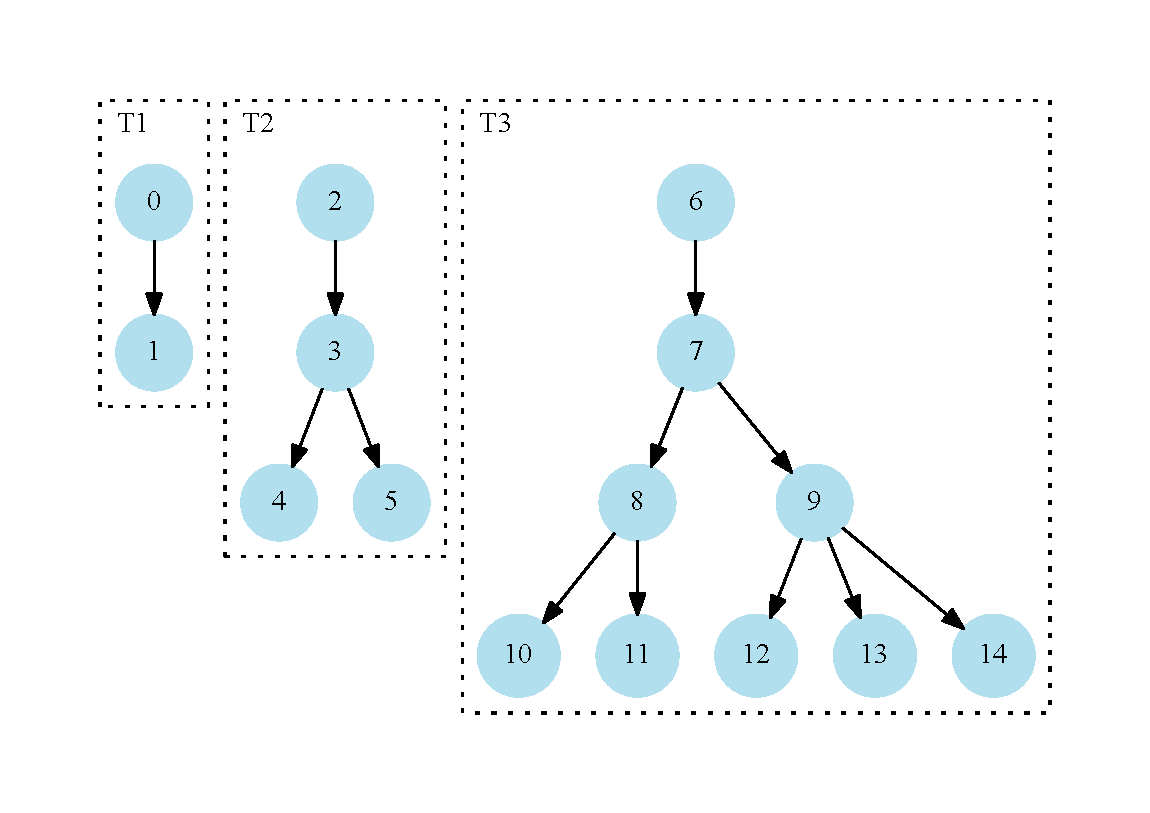
\includegraphics[scale=0.6]{./images/t1_2_3.pdf}
\end{center}
\caption{arborescences $\mathcal{T}_1$, $\mathcal{T}_2$, $\mathcal{T}_3$}
\end{figure}
\clearpage

\begin{figure}[h]
\begin{center}
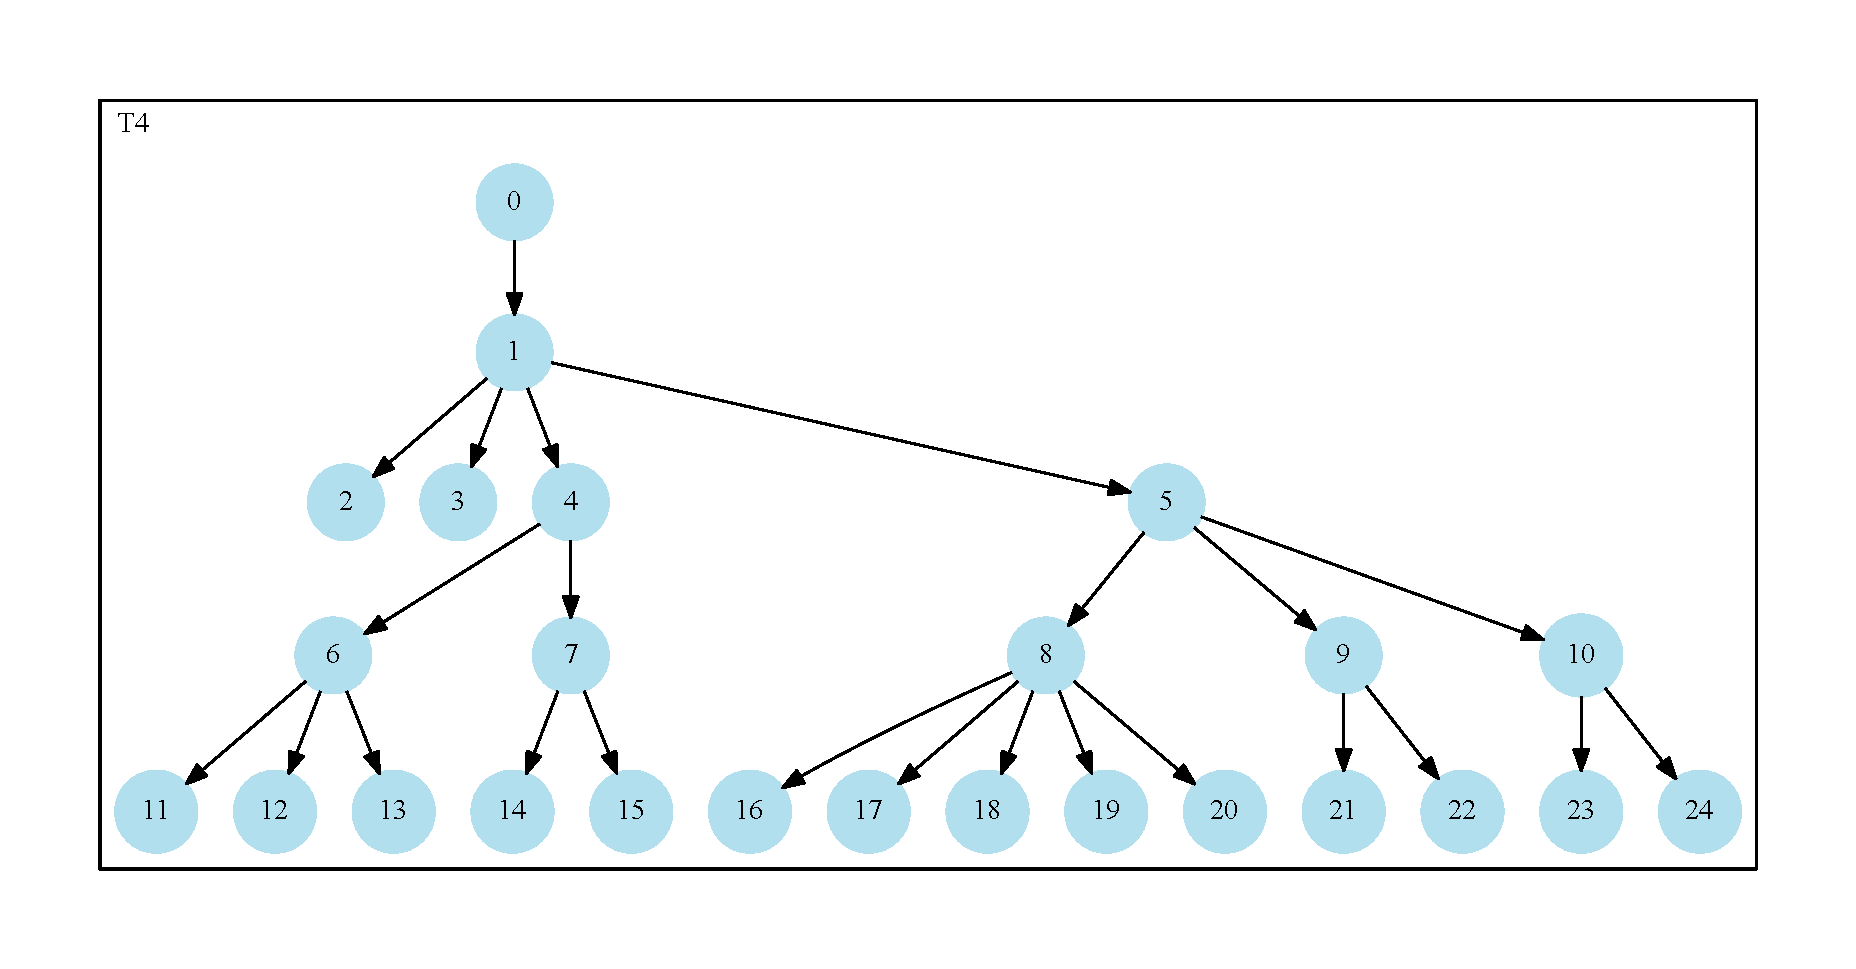
\includegraphics[scale=0.4]{./images/t4.pdf}
\end{center}
\caption{arborescence $\mathcal{T}_4$}
\end{figure}
\clearpage
%appendice B
\chapter{Programmation}

\begin{rem}[astuce -- trafic automobile]
En C/C++, on peut repr\'esenter une s\'equence de $n$ bits par un entier non sign\'e de type \verb+uint32_t+ dont on ne consid\`ere que les $n$ premiers bits \`a droite dans l'\'ecriture en base $2$. On peut alors coder $f$ facilement en utilisant des op\'erations de \og masques \fg{} (symboles \verb+&+, \verb+|+, \verb+!+, \verb+^+) et de d\'ecalage de bits (symboles \verb+<<+ et \verb+>>+) qui correspondent respectivement \`a des op\'erations logiques bit-\`a-bit et \`a des divisions/multiplications par des puissances de $2$. Nous renvoyons au code de la fonction $f$ qui tient en une seule ligne.
\end{rem}

L'exemple lin\'eaire et le trafic routier sont \'etudi\'es par des programmes \'ecrits respectivement en Python et en C/C++.

\end{document}